\documentclass[11pt,a4paper]{article}

\usepackage[margin=2.2cm]{geometry}
\usepackage{fontspec}
\usepackage{xeCJK}
\setmainfont{Times New Roman}
\setCJKmainfont{DFKai-SB}[AutoFakeBold,AutoFakeSlant]
\usepackage{amsmath,amssymb,bm}
\usepackage{graphicx}
\usepackage{caption}
\usepackage{wrapfig}
\usepackage{setspace}
\usepackage{hyperref}

\hypersetup{colorlinks=true,linkcolor=black,urlcolor=blue}
\captionsetup{font=small,labelfont=bf,skip=4pt}
\graphicspath{{figures/}}
\setstretch{1.08}
\raggedbottom
\setlength{\intextsep}{8pt plus 2pt minus 2pt}
\setlength{\textfloatsep}{10pt plus 2pt minus 2pt}
\setlength{\abovedisplayskip}{8pt}
\setlength{\belowdisplayskip}{8pt}

\title{\textbf{Control System Homework 01}\\[0.3em]
\large Unit 2: Dynamic Models\\[0.45em]
Problem~3 (2.19): Capacitor Microphone}
\author{許楷翊\\[2pt] B13901040}
\date{September 2026}

\begin{document}
\maketitle

This note models the capacitor microphone in Fig.~\ref{fig:schematic}, answers (a)--(c),
and shows why writing the electric force as \(f_e\operatorname{sgn}(\dot{x})\) is not physical.

%==============================================================================
\section{What the system is}

Plate \(a\) is fixed. Plate \(b\) (mass \(M\)) is held by a spring \(K\) and a damper \(B\).
Sound applies a force \(f_s(t)\) on \(b\). The two plates form a capacitor of gap \(x\),
wired in series with \(L\), \(R\), and a source \(v\).

\begin{wrapfigure}{r}{0.46\textwidth}
  \centering
  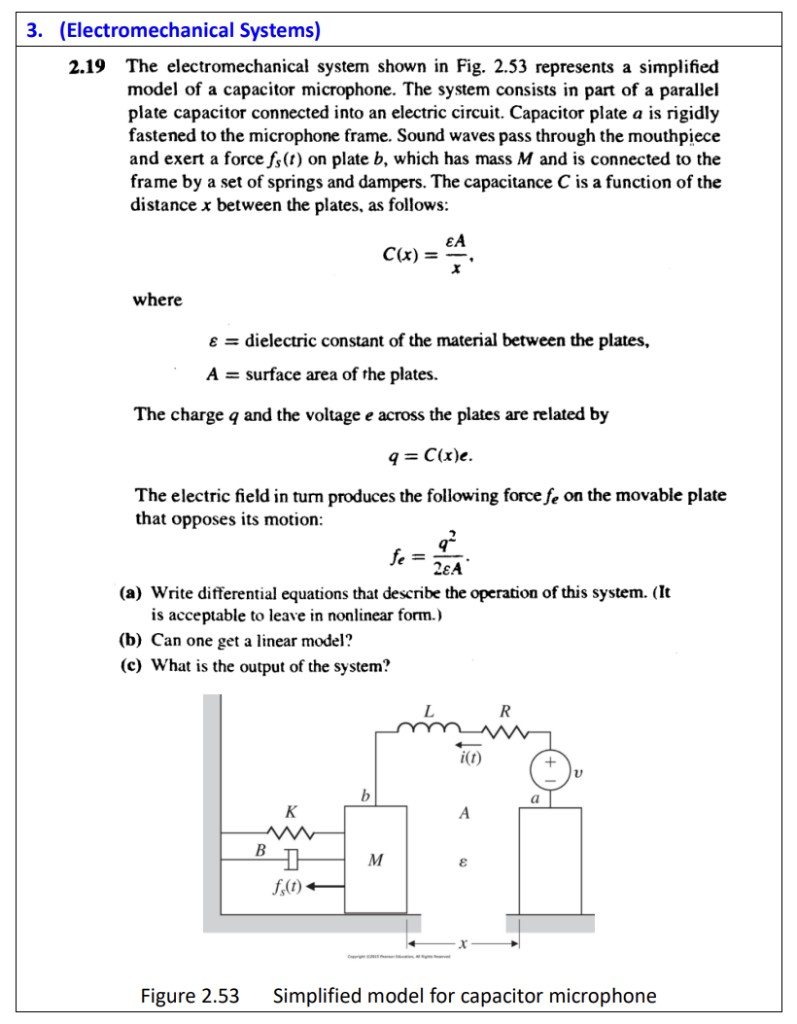
\includegraphics[width=0.44\textwidth]{fig_schematic.png}
  \caption{Fig.~2.53. Simplified capacitor microphone.}
  \label{fig:schematic}
\end{wrapfigure}

The problem gives
\begin{equation}
  C(x)=\frac{\varepsilon A}{x},\qquad
  q=C(x)\,e,\qquad
  f_e=\frac{q^2}{2\varepsilon A}.
\label{eq:given}
\end{equation}
A smaller gap means a larger capacitance. \(f_e\) is the electric force on the moving plate.
The text says this force ``opposes its motion.''

Coordinate: \(x\) is the gap. Increasing \(x\) means \(b\) moves left and the plates separate.
\(f_s>0\) increases \(x\). The source is a DC bias \(V_0\) (a real condenser microphone also needs bias
to turn motion into an electrical signal).

%==============================================================================
\section{Which way does \(f_e\) point?}
\label{sec:fe}

This circuit is one capacitor: \(b\) carries \(+q\), \(a\) carries \(-q\).
The plates always have opposite charge. The force depends on \(q^2\), so
\[
f_e=\frac{q^2}{2\varepsilon A}\ge 0.
\]
Opposite charges attract: \(f_e\) always pulls \(b\) toward \(a\), so it always
\textbf{decreases} \(x\). The direction does not depend on \(\dot{x}\).
If \(q=0\) the force is zero; it never becomes a repulsion.

The official solution (Fig.~\ref{fig:fbd}) instead writes
\begin{equation}
  M\ddot{x}+B\dot{x}+Kx+f_e\operatorname{sgn}(\dot{x})=f_s(t),
\label{eq:sgn}
\end{equation}
which reads ``opposes its motion'' as ``always against the velocity.''
That is friction, not electrostatic attraction.

\begin{figure}[ht]
  \centering
  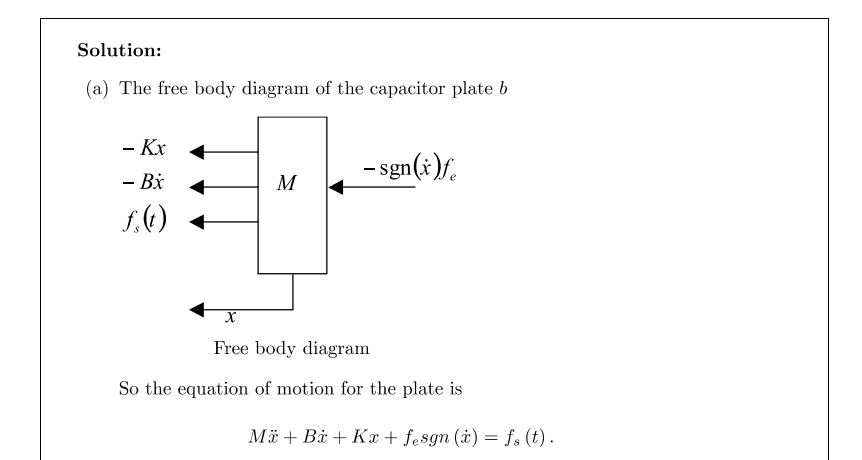
\includegraphics[width=0.42\textwidth]{fig_fbd_sol.png}
  \caption{Solution FBD: \(f_e\) is multiplied by \(\operatorname{sgn}(\dot{x})\).}
  \label{fig:fbd}
\end{figure}

Three problems:
\begin{enumerate}
  \item \textbf{A charged capacitor still pulls at rest.}
        \(\operatorname{sgn}(0)=0\), so the force vanishes whenever the plate stops.
  \item \textbf{Closing should attract, not push.}
        When \(\dot{x}<0\) (gap shrinking), \eqref{eq:sgn} becomes a repulsion.
  \item \textbf{This force is conservative, not a damper.}
        Pulling the plates apart takes work; letting them close, the field does work.
        Power can be positive or negative. \(\operatorname{sgn}\) makes the power always \(\le 0\).
\end{enumerate}

A better reading of ``opposes its motion'' is: \textbf{you must overcome attraction to separate the plates},
not that the force always points against \(\dot{x}\).

So the correct mechanics equation is
\begin{equation}
  M\ddot{x}+B\dot{x}+K\bigl(x-x_{\mathrm{rest}}\bigr)+f_e=f_s(t),
\label{eq:mech}
\end{equation}
where \(f_e\) always shrinks the gap. \(x_{\mathrm{rest}}\) is the gap when the spring is unstretched.

%==============================================================================
\section{Circuit}

KVL around the loop (source, resistor, inductor, capacitor) gives
\begin{equation}
  L\dot{i}+Ri+e=V_0,\qquad
  e=\frac{qx}{\varepsilon A},\qquad
  i=\dot{q}.
\label{eq:kvl}
\end{equation}

%==============================================================================
\section{(a) Nonlinear equations}

With state \((x,\dot{x},q,i)\),
\begin{equation}
\begin{aligned}
  \ddot{x}&=\frac{1}{M}\Bigl[f_s(t)-\frac{q^2}{2\varepsilon A}
           -K\bigl(x-x_{\mathrm{rest}}\bigr)-B\dot{x}\Bigr],\\
  \dot{q}&=i,\\
  \dot{i}&=\frac{1}{L}\Bigl(V_0-Ri-\frac{qx}{\varepsilon A}\Bigr).
\end{aligned}
\label{eq:nlin}
\end{equation}
The VPython simulation integrates \eqref{eq:nlin} as is, without linearizing.

%==============================================================================
\section{(b) Can we linearize?}

Yes, but only near the \textbf{biased equilibrium}, for a small sound force.

With \(f_s=0\) and zero velocity and current, the rest point \((x_0,q_0)\) satisfies
\begin{equation}
  q_0=\frac{\varepsilon A V_0}{x_0},\qquad
  K(x_0-x_{\mathrm{rest}})+\frac{q_0^2}{2\varepsilon A}=0.
\label{eq:eqpt}
\end{equation}
The spring must balance a constant attraction, so \(x_0<x_{\mathrm{rest}}\)
(the plates sit closer than with no voltage). The \(\operatorname{sgn}\) model has \(f_e=0\) at rest,
so it wrongly puts the equilibrium at \(x_{\mathrm{rest}}\).

Let \(x=x_0+\delta x\), \(q=q_0+\delta q\). Dropping second-order terms,
\begin{equation}
\begin{aligned}
  M\delta\ddot{x}+B\delta\dot{x}
  +\Bigl(K-\frac{q_0^2}{\varepsilon A x_0^2}\Bigr)\delta x
  +\frac{q_0}{\varepsilon A}\,\delta q
  &=\delta f_s,\\
  L\delta\ddot{q}+R\delta\dot{q}
  +\frac{x_0}{\varepsilon A}\,\delta q
  +\frac{q_0}{\varepsilon A}\,\delta x
  &=0.
\end{aligned}
\label{eq:lin}
\end{equation}
Electrostatics soften the spring. For a small input, \eqref{eq:nlin} looks like \eqref{eq:lin};
if the input is large the motion is nonlinear and can pull in.

The official solution says the \(\operatorname{sgn}\) function together with the \(q^2\) and \(qx\) terms
make a useful linear model impossible. These should not be lumped together.
\(\operatorname{sgn}(\dot{x})\) is not differentiable at \(\dot{x}=0\), so a standard Jacobian linearization fails.
The terms \(q^2\) and \(qx\) are smooth. About a biased point with \(q_0\neq 0\),
\[
\delta(q^2)=2q_0\delta q,\qquad
\delta(qx)=q_0\delta x+x_0\delta q,
\]
which is exactly \eqref{eq:lin}. Linearizing at \(q=0\) does kill the first-order coupling, and a microphone
with no bias would indeed have no useful small-signal output.
So dropping \(\operatorname{sgn}\) is necessary, but one must also expand about \((x_0,q_0)\).

%==============================================================================
\section{(c) What is the output?}

The output is the current \(i(t)\) (or the voltage \(Ri\)), not the gap \(x\).
Under bias, \(q\approx C(x)V_0\), so
\begin{equation}
  i=\dot{q}\approx -\frac{\varepsilon A V_0}{x^2}\,\dot{x}.
\label{eq:i}
\end{equation}
Thus \(i\) tracks \textbf{velocity}:
\begin{itemize}
  \item step: \(x\) settles to a new gap, then \(i\to 0\) (no DC gain);
  \item impulse: \(x\) rings back; \(i\) is nonzero only while the plate moves;
  \item sine: both \(x\) and \(i\) keep oscillating.
\end{itemize}
A capacitor microphone only responds to a \emph{changing} pressure.

%==============================================================================
\section{Simulation}

We integrate \eqref{eq:nlin} with Euler (semi-implicit on the current).
Parameters are scaled so the motion is visible; the equations are the same as in the problem.
The input \(f_s\) can be a step, a short pulse (impulse), or a sine.

\subsection{Impulse}

Fig.~\ref{fig:impulse}: a pulse at \(t=1\,\mathrm{s}\). \(x\) leaves equilibrium and returns.
\(i\) is a pulse, then zero---same shape as \(\dot{x}\). The cyan \(f_e\) stays almost constant
(always an attraction).

\begin{figure}[ht]
  \centering
  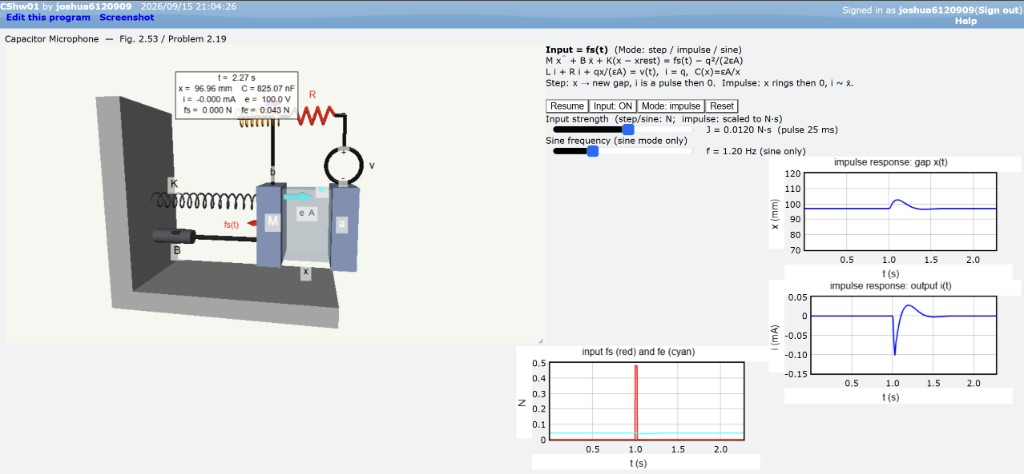
\includegraphics[width=0.88\textwidth,height=0.28\textheight,keepaspectratio]{fig_impulse.png}
  \caption{Impulse response: \(x\) rings back; \(i\) is nonzero only during motion.}
  \label{fig:impulse}
\end{figure}

\subsection{Sine}

Fig.~\ref{fig:sine}: after \(t=1\,\mathrm{s}\), \(f_s\) is sinusoidal. Both \(x\) and \(i\) oscillate.
\(f_e\) is almost a flat line; it does not flip when velocity changes sign.

\begin{figure}[ht]
  \centering
  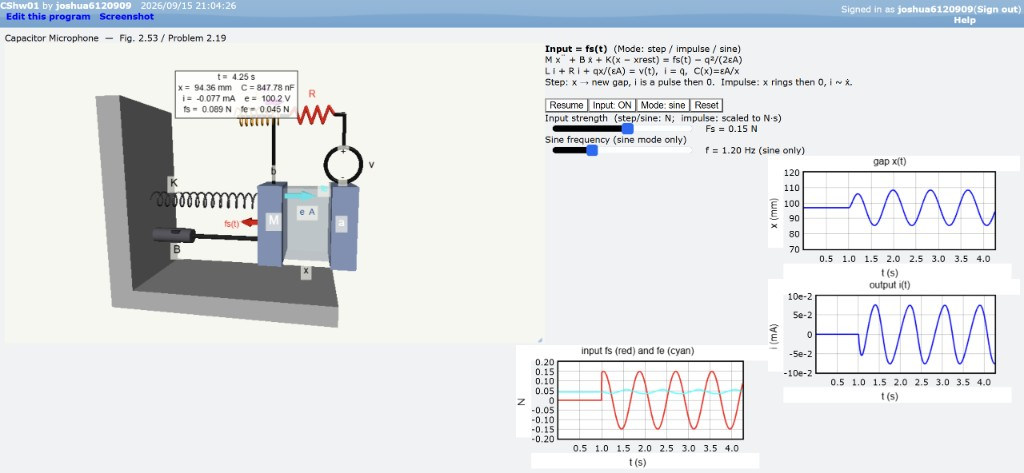
\includegraphics[width=0.88\textwidth,height=0.28\textheight,keepaspectratio]{fig_sine.png}
  \caption{Sine input. Red: \(f_s\). Cyan: \(f_e\) (almost constant). Right: \(x\) and \(i\).}
  \label{fig:sine}
\end{figure}

%==============================================================================
\section{Comparison with the \(\operatorname{sgn}\) model}

Same \(f_s\), same circuit; only the mechanical force law changes:
\begin{align}
  \text{physics (blue)}&\quad
  M\ddot{x}+B\dot{x}+K(x-x_{\mathrm{rest}})+f_e=f_s,
  \label{eq:phys}\\
  \text{solution (orange)}&\quad
  M\ddot{x}+B\dot{x}+K(x-x_{\mathrm{rest}})+f_e\operatorname{sgn}(\dot{x})=f_s.
  \label{eq:sol}
\end{align}
Both runs start charged and at rest at \(x_{\mathrm{rest}}\).
\(F_{x,e}\) is the electric force along \(+x\) (opening the gap). In physics it should stay negative.

\subsection{Step: orange has no force at rest}

Fig.~\ref{fig:cstep}, first \(1.5\,\mathrm{s}\) with no sound:
\begin{itemize}
  \item Blue: attraction starts at once; \(x\) falls from \(100\,\mathrm{mm}\) to about \(97\,\mathrm{mm}\).
  \item Orange: \(\operatorname{sgn}(0)=0\), so \(F_{x,e}=0\) and the plate stays at \(100\,\mathrm{mm}\).
\end{itemize}
The plates are charged, yet the orange model does not move. The step is applied only after \(1.5\,\mathrm{s}\).

\begin{figure}[ht]
  \centering
  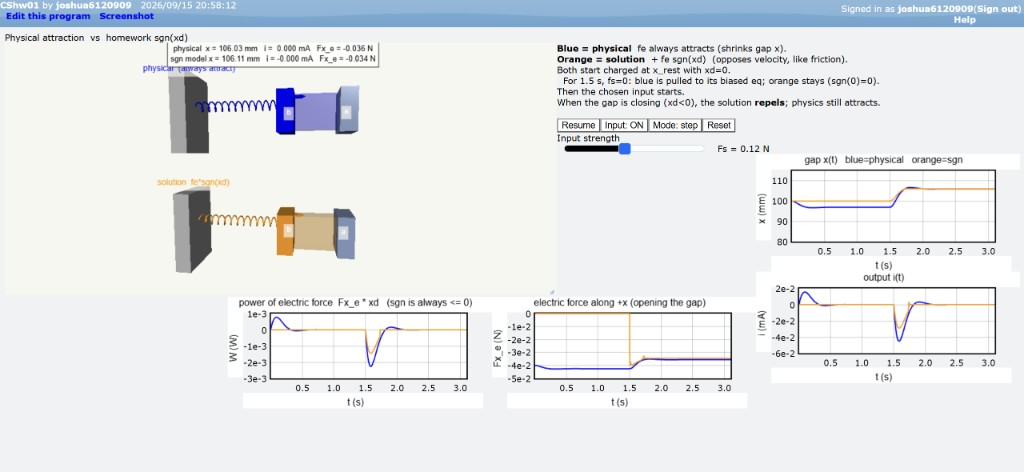
\includegraphics[width=0.88\textwidth,height=0.28\textheight,keepaspectratio]{fig_compare_step.png}
  \caption{Blue $=$ physics, orange \(=\operatorname{sgn}\). For \(t<1.5\,\mathrm{s}\) blue is pulled in; orange is not.}
  \label{fig:cstep}
\end{figure}

\subsection{Sine: the force should not follow velocity}

Fig.~\ref{fig:csine}:
\begin{itemize}
  \item \(x\): blue oscillates about a closer gap; orange stays near \(100\,\mathrm{mm}\) (no preload).
  \item \(F_{x,e}\): blue is almost a negative DC (always attracting); orange is modulated by \(\dot{x}\) and often returns to 0.
  \item \(i\): orange is larger, because the mean gap and the force law are both wrong, so the output is wrong too.
\end{itemize}

\begin{figure}[ht]
  \centering
  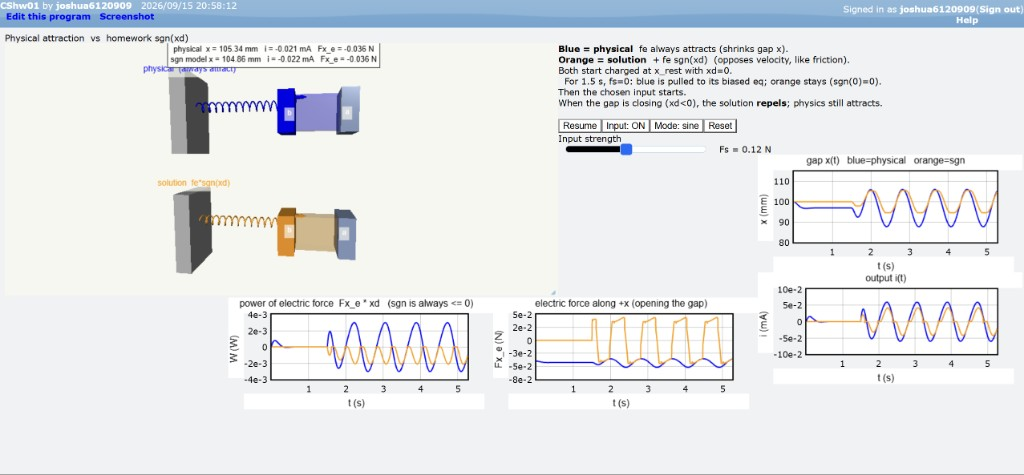
\includegraphics[width=0.88\textwidth,height=0.28\textheight,keepaspectratio]{fig_compare_sine.png}
  \caption{Sine comparison. Blue \(F_{x,e}\) stays negative; orange tracks velocity, like friction.}
  \label{fig:csine}
\end{figure}

A hard \(\operatorname{sgn}\) also chatters when the speed crosses zero.
A true Coulomb attraction should not do that.

%==============================================================================
\section{Conclusion}

\begin{enumerate}
  \item \textbf{(a)} Use \eqref{eq:nlin}: a mass--spring--damper with a one-way attraction,
        plus an \(L\)--\(R\)--\(C\) circuit whose \(C\) depends on \(x\).
  \item \textbf{(b)} Linearization is possible after dropping \(\operatorname{sgn}\), at the biased point \((x_0,q_0)\).
        \(q^2\) and \(qx\) are ordinary smooth nonlinearities; the solution overstates that they cannot be linearized.
  \item \textbf{(c)} The output is \(i(t)\). No steady current for a DC pressure; for AC, \(i\propto \dot{x}\).
  \item \(f_e\operatorname{sgn}(\dot{x})\) disagrees with \(f_e=q^2/(2\varepsilon A)\):
        opposite charges always attract. The simulation shows no force at rest in the \(\operatorname{sgn}\) model,
        and a velocity-dependent \(F_{x,e}\) under sine input.
\end{enumerate}

Read ``opposes its motion'' as ``attraction must be overcome to open the gap.''
Use \eqref{eq:mech}, not \eqref{eq:sgn}.

\vspace{0.6em}
\noindent Programs: \texttt{capacitor\_microphone.py} (physics),
\texttt{capacitor\_microphone\_sgn\_compare.py} (comparison).

\end{document}
